\chapter{Generative Adversarial Networks}
\label{chap:chapter1}

\begin{chapterabstract}
	In this chapter, we propose an overview	 of the Generative Adversarial Networks \cite{Goodfellow2014} framework, some of its theoretical interpretations, as well as some of its variations and applications. We discuss the different limitations of this approach and expose a trilemma between the quality of the generated samples, their diversity and the conditioning of the model. We then discuss the recent advances that have been made to overcome some of these limitations and propose a classification of these advances using the aforementioned trilemma. Finally, we discuss the evaluation of generative models and the difficulties of evaluating the intrinsic quality of a generated sample.  We propose an overview of the different classical metrics and discuss their limitations.
\end{chapterabstract}

\minitoc

\section{Generative Adversarial Networks}

In this section, we introduce the Generative Adversarial Networks \cite{Goodfellow2014}.  We will first 

\subsection{The GAN framework}

GAN formulation, loss variations, JS/KL interpretation of the loss

\subsection{Conditional modeling with  \ac{GAN}}
Conditional GANs

Introduction to domain-transfer (Pix2Pix, CycleGAN) through removal of the random noise

\section{Limitations}

Image quality : Incremental enhancement through architecture, more data, ... 

Instability, catastrophic forgetting and the mode collapse problem

Trade-off image quality/diversity : Explanation through the loss term and distribution coverage

Black-box approach to conditioning, no tuning possible, no interpretability

\section{The GAN Zoo}

\subsection{A taxonomy of GANs}
Enorme nombre de variantes de GANs

Taxonomie des approches GANs (pour s'éviter une liste des différents GANs)

Schéma pour définir les grandes familles de GAN (évoquer les AmbientGAN / UNIR)

\subsection{Architecture variants}

\subsection{Divergence variants}
Table des loss alternatives (f-divergences + transport optimal)

\subsection{Task-specific losses}

\begin{figure}
	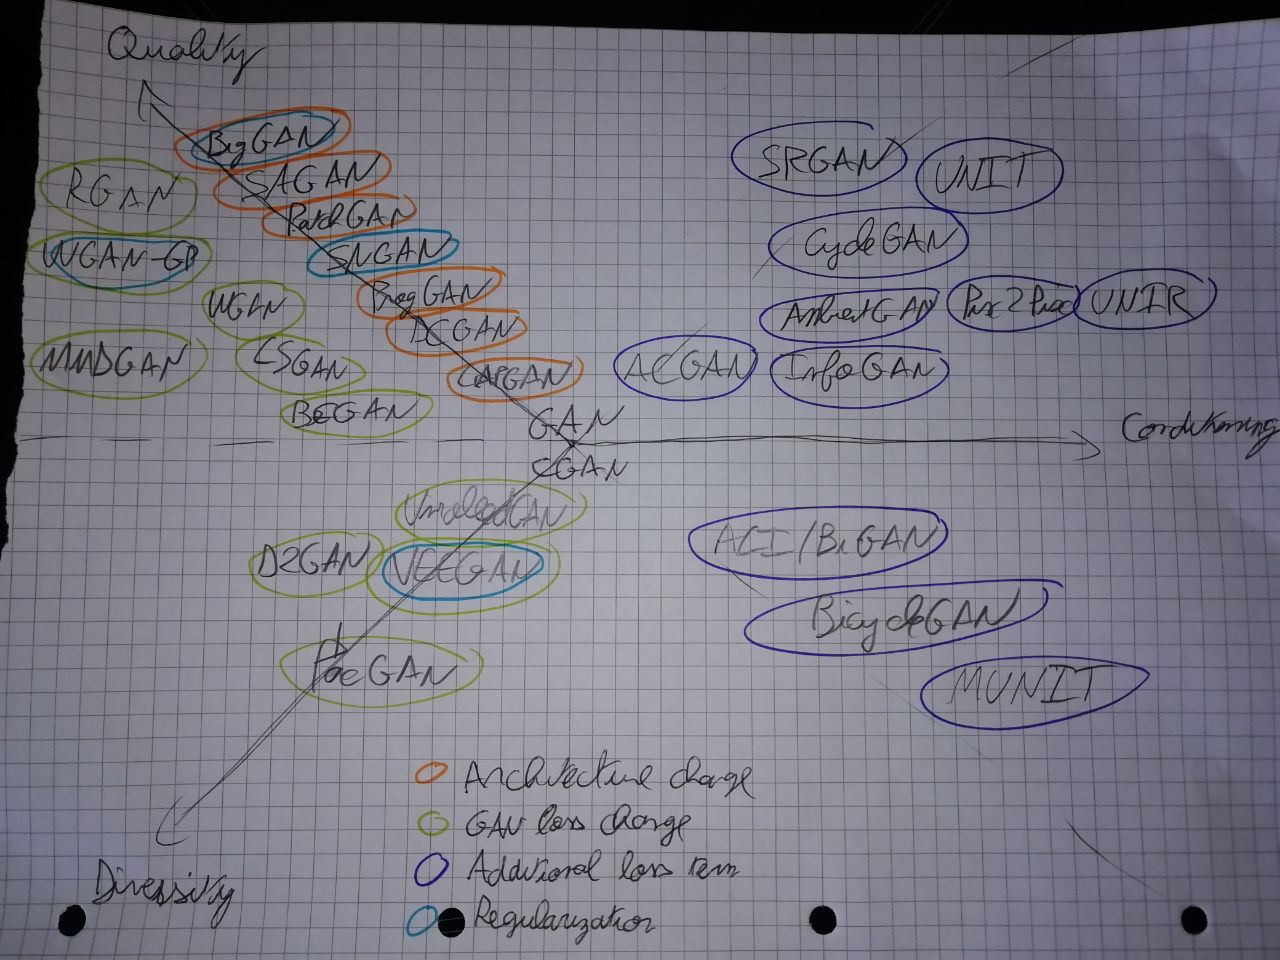
\includegraphics[width=\textwidth]{chapter1/trilemma.jpg}
	\caption{Classifications of some advances in GANs on the trilemma}
\end{figure}

\section{A note on the  evaluation of generative models}

No good adhoc methods

Image quality : Inception distance + Fréchet inception distance, advantages

Conditioning : Direct evaluation (pixel-wise), Classifier accuracy, Projections (PCA, t-SNE)

Limitations of those metrics : need a pre-trained model


